\chapter{基于pthread的形态学图像处理}
\section{实验目的与要求}
\begin{itemize}
    \item 掌握使用pthread的基本的并行编程设计方法以及调优方法;
    \item 掌握并行编程中基本的数据分块以及任务分解的方法。
    \item 使用pthread实现并行的形态学图像处理。
    \item 简要分析以及总结处理的结果。
\end{itemize}

\section{算法描述}
\par 使用多个线程对于一个图像进行蚀刻以及膨胀的算法如下,算法为一个线程的流程,而有多个这样的线程同时进行。
\begin{simpleAlgorithm}{pthread并行处理算法(一个线程)}
    \Procedure{PthreadParallel}{$blocks$}
    \While{true}
        \State lock\((blocks)\)
        \State get first block \(blk\) from \(blocks\)
        \If{\(blocks\).empty()}
            \State unlock\((blocks)\)
            \State \Return
        \EndIf
        \State unlock\((blocks)\)
        \State \Call{ErodeAndDilate}{$blk, kernel_e, kernel_d$}
    \EndWhile
    \EndProcedure
\end{simpleAlgorithm}
\par 算法中,\(blocks\)参数为一个工作队列,队列中的工作为原预处理过后的图片的子图片。在每个线程的每个循环中,首先锁住队列,从队列中获取一个子图片\(blk\)、解锁队列然后使用上一章中的ErodeAndDilate过程进行处理。如果\(blocks\)中没有子图片,说明处理完成,则此线程退出。
\par 主线程的流程如图\ref{fig:pthreadMain}所示。在进行预处理过后启动多个线程,然后等待所有线程竞争子图像、处理然后结束即可,最后保存处理的结果即可。
\begin{figure}[htpb]
    \centering
    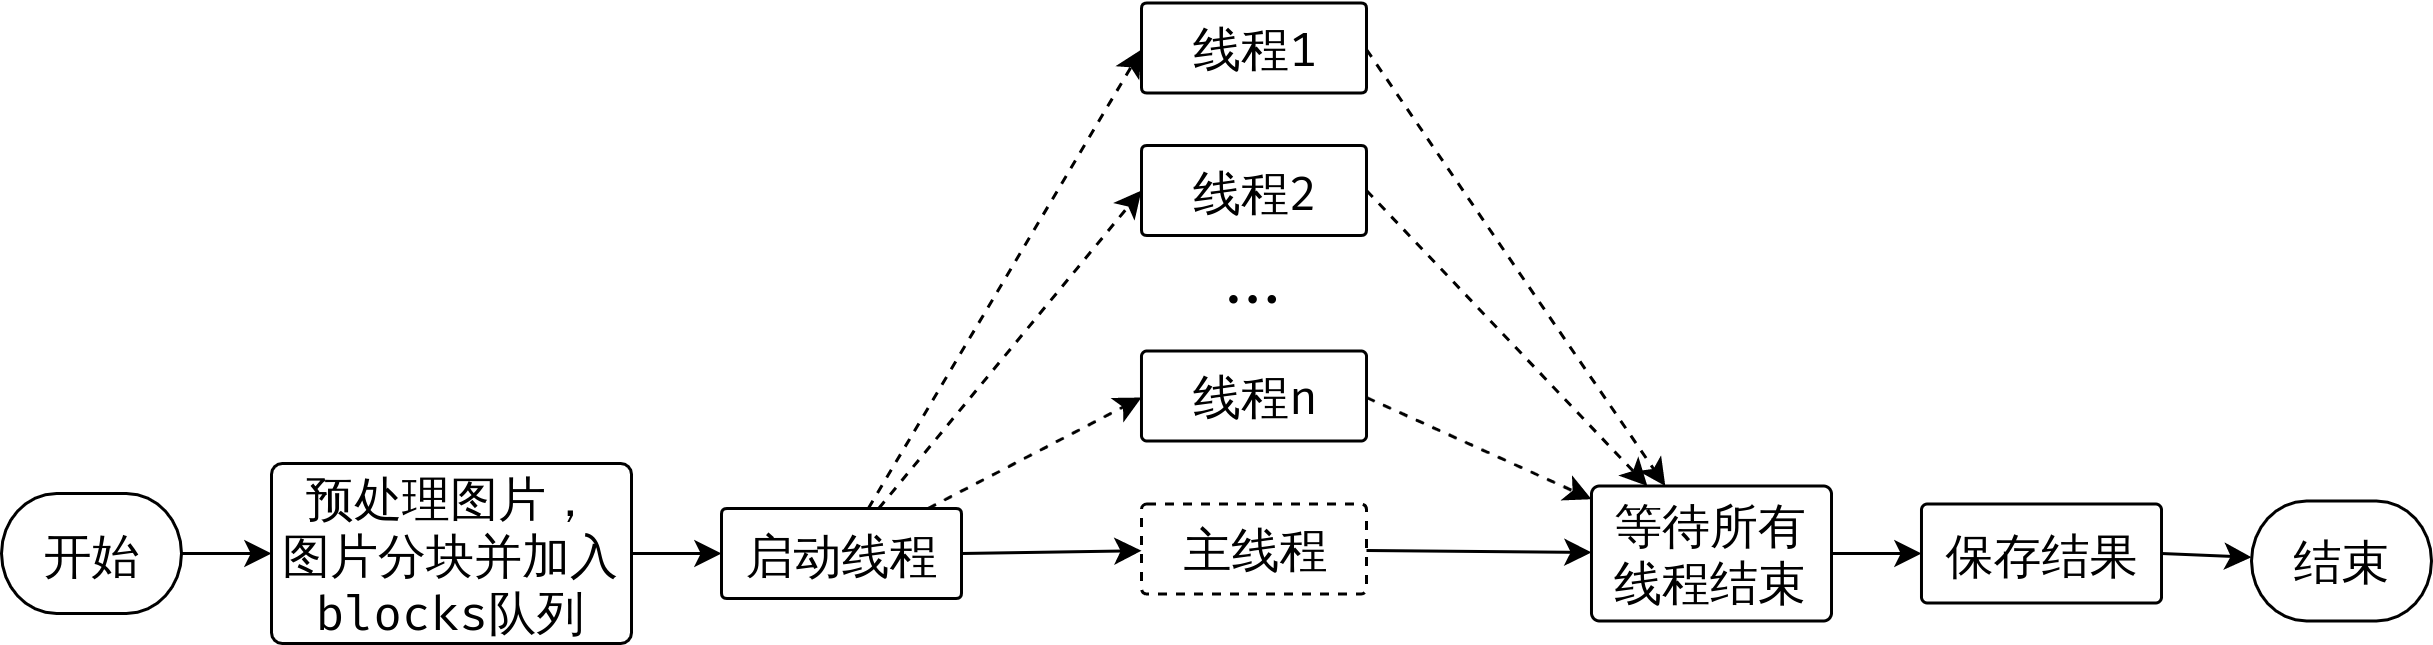
\includegraphics[width=0.95\linewidth]{pthreadMain.png}
    \caption{主线程流程}
    \label{fig:pthreadMain}
\end{figure}

\par 由于是使用pthread的并行算法,每一个线程处理一个部分,因此首先需要将数据分块(即分为算法中的\(blocks\))。分块方式如图\ref{fig:partition}所示。每块大小一样,在边缘部分如果块大小不符则按照原图的边缘进行裁减。因此,在进行处理时需要对于边缘部分进行考虑。
\begin{figure}[htpb]
    \centering
    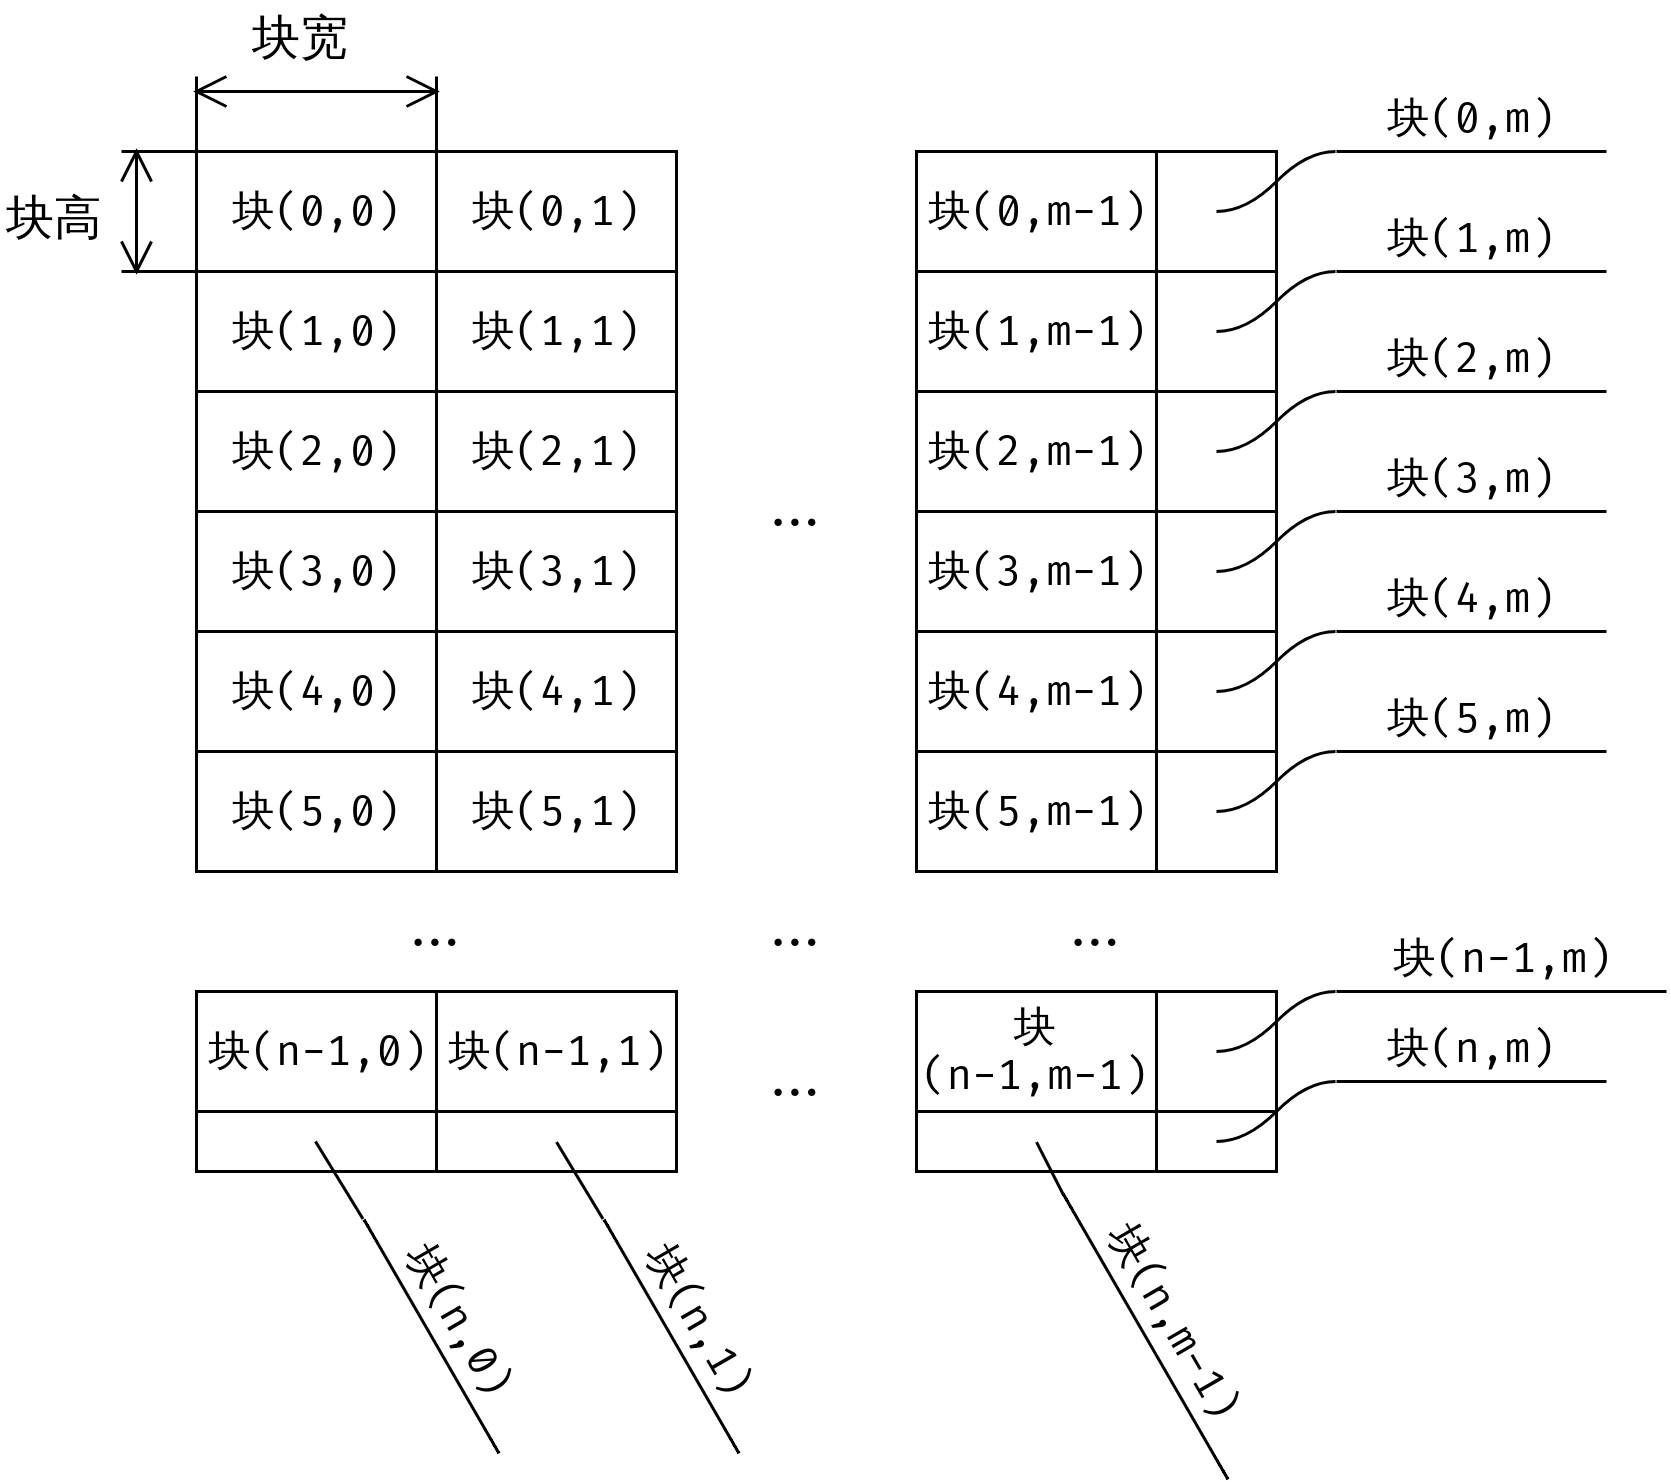
\includegraphics[width=0.76\linewidth]{partition.png}
    \caption{分块方法}
    \label{fig:partition}
\end{figure}

\section{实验方案}
\par 所有的开发与运行环境见附录\ref{cha:env},表\ref{tab:env},此后实验的开发与运行环境均相同,不再赘述。根据算法描述、分块方法以及主线程的流程编写程序并运行,然后观察结果并与串行的程序比较。经过多轮的比较以及参数调试后得出一个较好的效果。

\section{实验结果与分析}
\par 功能上,程序处理后的图片与串行处理后的图片一致,此处不再给出。4线程,分块大小为128的情况下程序的运行时间如图\ref{fig:pthreadOutput}所示。在4个线程的情况下,运行三次的平均运行时间为11.7s,相比于串行算法,程序的加速比为\(44.2\div 11.7 = 3.77\),已经十分接近理想加速比4。
\begin{figure}[htpb]
    \centering
    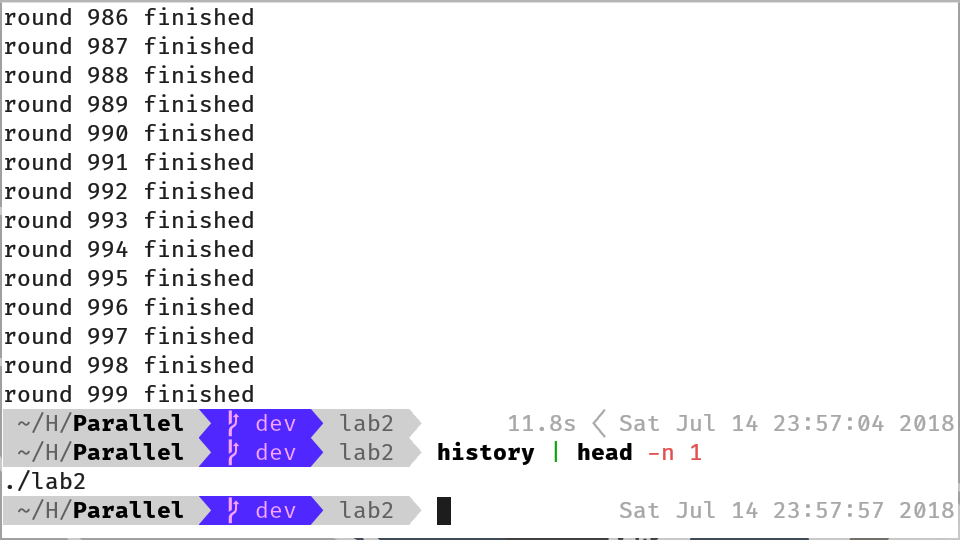
\includegraphics[width=0.9\linewidth]{pthreadOutput.png}
    \caption{pthread程序运行时间}
    \label{fig:pthreadOutput}
\end{figure}

\par 经过8组、每组3次的测试,加速比随线程变化的曲线如图\ref{fig:pthreadTrend}所示。可以看出,在线程数为1\textasciitilde 4时加速比随着线程数几乎呈线性变化,而在线程数为1时加速比为1.006,overhead所占用的时间几乎可以不计。在线程数达到4时由于物理内核已经被占满,因此后面加速比不再增加,随着线程数量的进一步增大,由于线程调度的开销,因此程序的加速比不再增加,反而有所下降。
\begin{figure}[htpb]
    \centering
    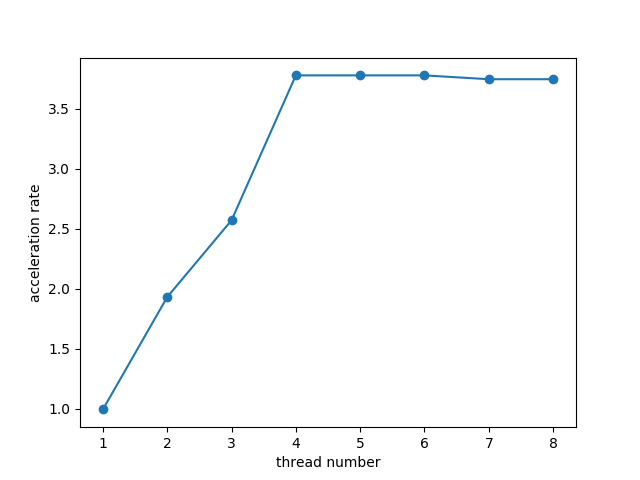
\includegraphics[width=0.8\linewidth]{pthreadTrend.png}
    \caption{加速比随线程数变化}
    \label{fig:pthreadTrend}
\end{figure}

\par 对于分块大小而言,加速比随着分块大小的变化如图\ref{fig:pthreadTrend2}所示,在分块大小较小时,加速比随着分块大小的变化并不大,只在分块大小过小时由于线程调度导致一点性能开销。当分块大小大于原图的一半时总时间则取决于分到最大分块线程所用的时间,因此在这个区间内性能随分块大小呈下降趋势。
\begin{figure}[htpb]
    \centering
    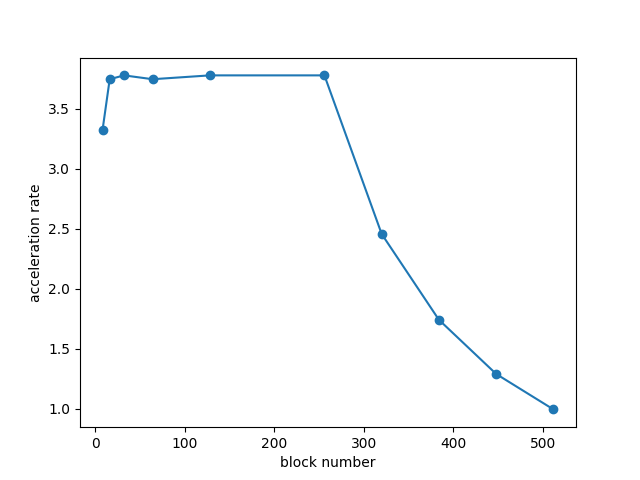
\includegraphics[width=0.8\linewidth]{pthreadTrend2.png}
    \caption{加速比随分块大小变化}
    \label{fig:pthreadTrend2}
\end{figure}


